\subsection{Driver}

The converter was not working properly in boost mode. However, it was possible to get some test results from it before failure. 
When this happened the driver of MOSFET 4 broke and needed to be changed. The reason is still being analyzed. 
Voltage spikes were found at the gate of the MOSFET which may be leading to failure. Figure \ref{Voltagespike} shows the output voltage of the driver after the gate resistors R11 and R12:

\begin{figure}[H]
	\begin{center}
		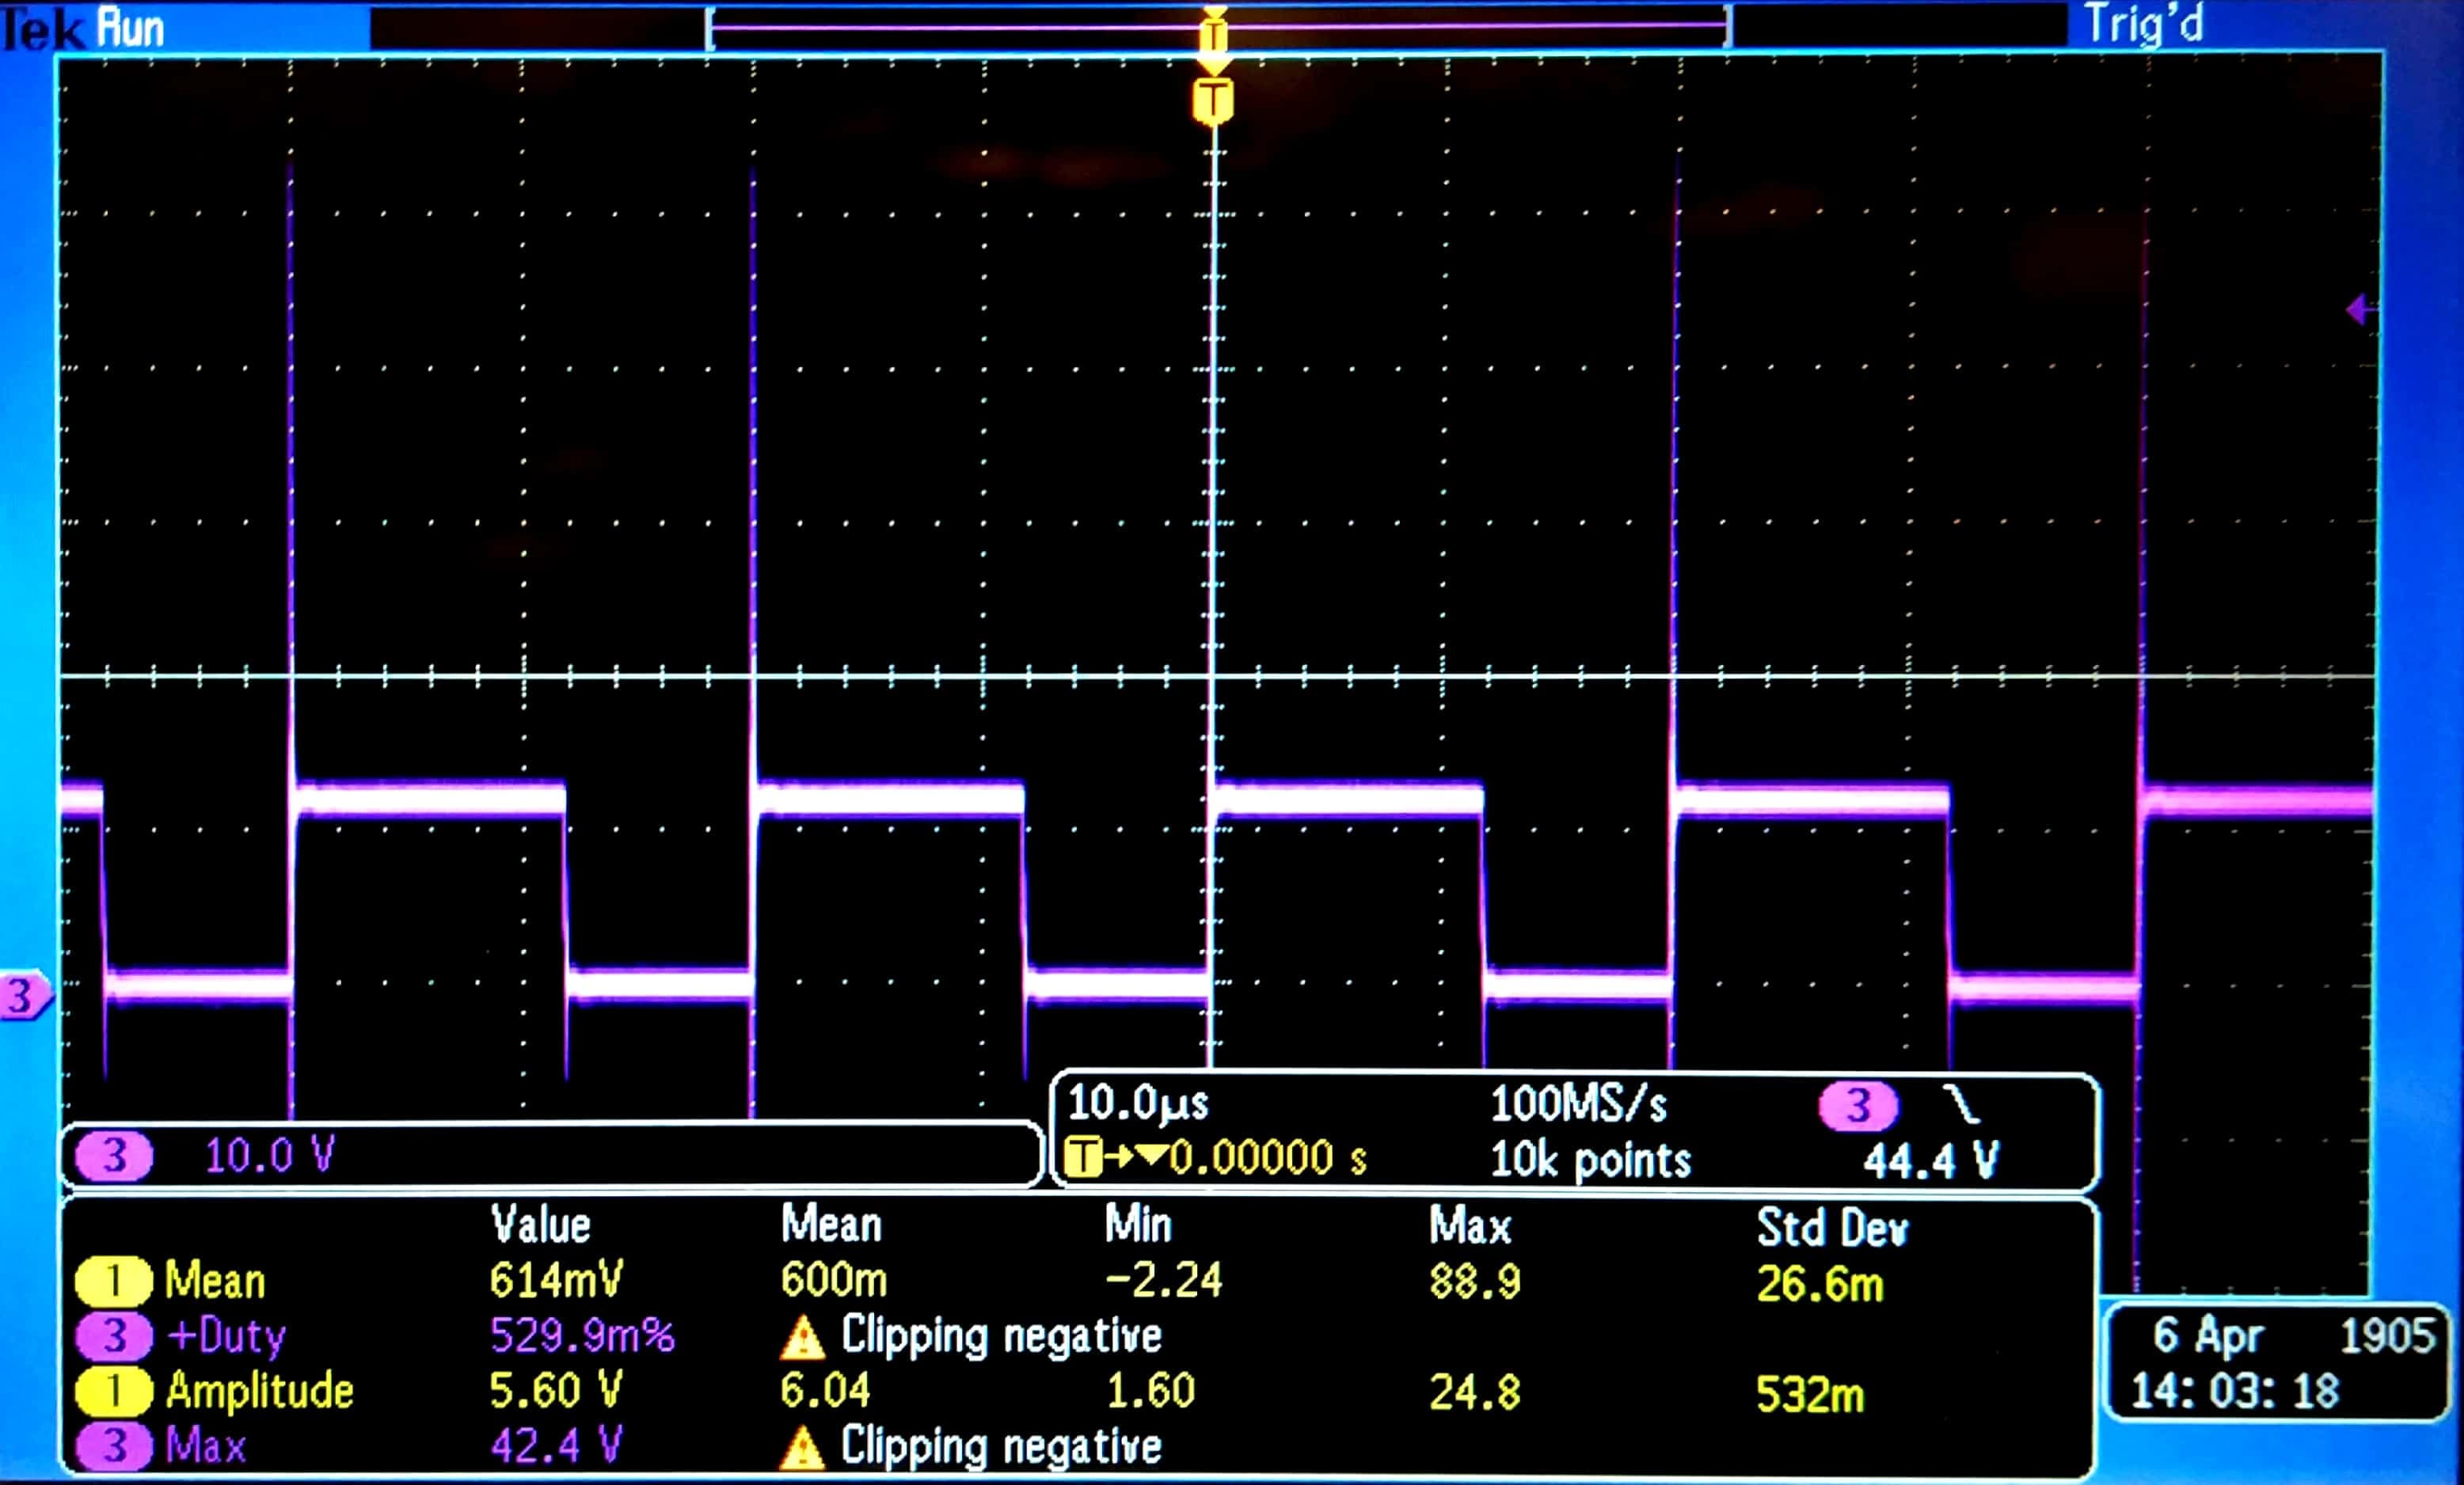
\includegraphics[width=0.7\textwidth]{../Pictures/P1/Discussion/Voltagespike.jpg}
		\caption{Voltage at the gate of MOSFET 4}
		\label{Voltagespike}
	\end{center}	
\end{figure}    

Looking at the figure, it can be seen that the switching spikes are reaching above 50V. This means that a large current will flow through the driver and MOSFET while switching which might be the cause of the driver failures. In an attempt to lowering these voltage spikes, the gate resistors were changed from $20\Omega$ to $100\Omega$. Improvements were obtained and are shown in figure \ref{Voltagespike_100}.
The drawback of increasing the gate resistors is an increase of the response time at the gate of the MOSFET. This behavior can also be seen in the figure.

\begin{figure}[H]
	\begin{center}
		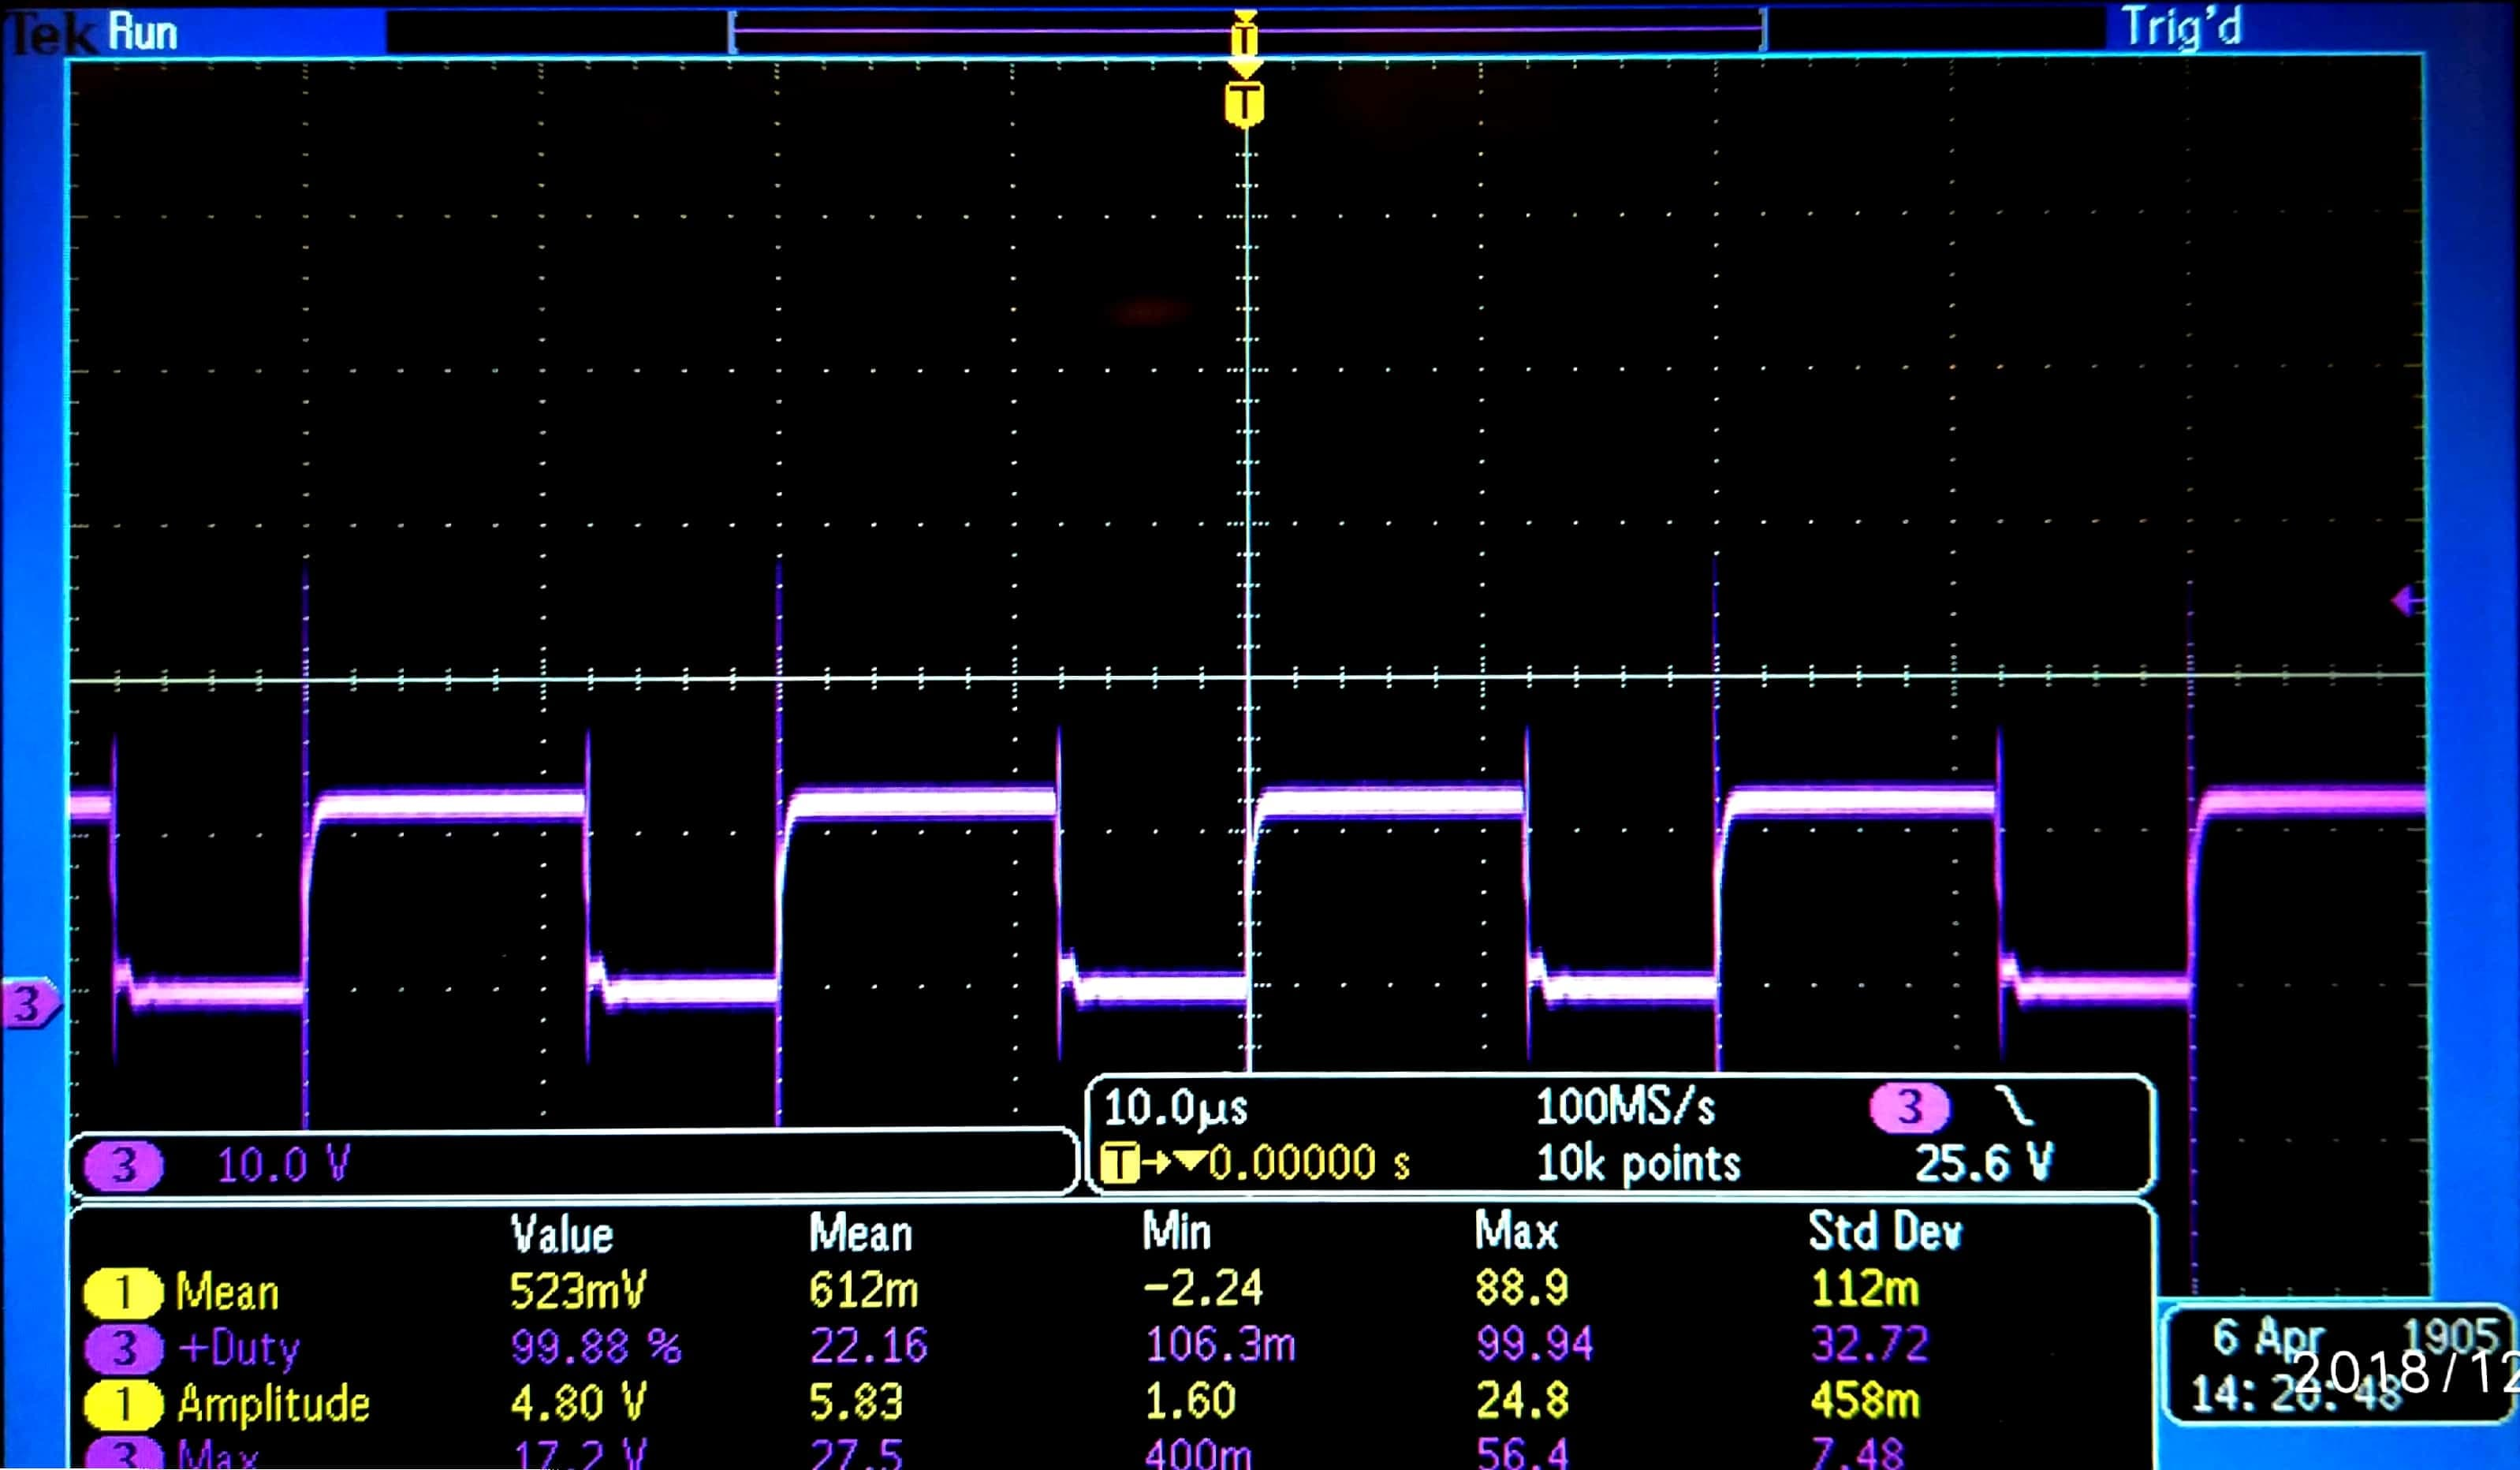
\includegraphics[width=0.7\textwidth]{../Pictures/P1/Discussion/Voltagespike_new_resistors.jpg}
		\caption{Output voltage of driver after gate resistors $100\Omega$}
		\label{Voltagespike_100}
	\end{center}	
\end{figure} 

As expected, the changed resistors have decreased the voltage spikes significantly. However, this did not solve the problem since the driver were still breaking. 